\subsection{Problem~11}%
\label{problem:11}

Digitalize a picture into a 640 x 400 (standard VGA) matrix of greyscale pixels, where the value of each pixel is a number $x: 0\leq{}x\leq1$; with black corresponding to $x=0$ and white to $x=1$.
Compute the SVD of this image matrix and display various approximations using 10; 20 and 40 of the singular values and vector pairs.
Do any of these give a good visual approximation of the image?
If not, find a minimal number that works.


\subsubsection*{Solution}
\lstinputlisting[style=Matlab-editor, breaklines=false]{problems/problem_11.m}
\subsection*{The results}
Independent variable was the number of singular values and vector pairs (10, 20, 40, 60, 80, 100). The results are as follows:
\begin{figure}[h]
    \centering
    
\includegraphics[width=0.5\linewidth]{figs/student_rat.png}
    \caption{Original}
    \label{fig:orginal}
\end{figure}
\begin{figure}[h]
    \centering
    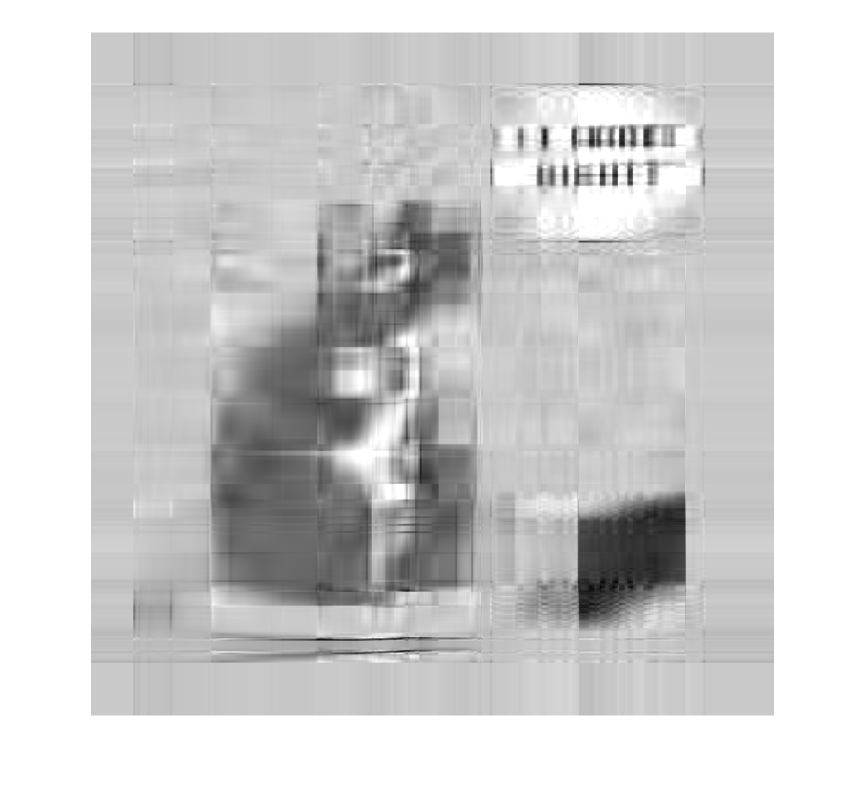
\includegraphics[width=0.5\linewidth]{figs/10_s_v.png}
    \caption{Image output using 10 singular values}
    \label{fig:10_s}
\end{figure}
\begin{figure}[h]
    \centering
    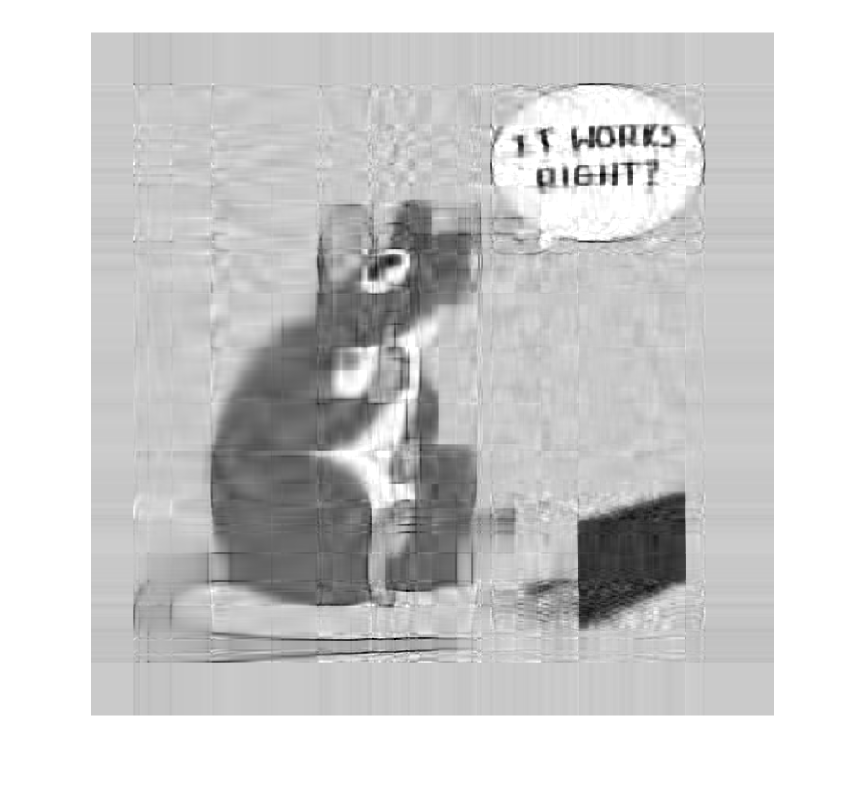
\includegraphics[width=0.5\linewidth]{figs/20_s_v.png}
    \caption{Image output using 20 singular values}
    \label{fig:20_s}
\end{figure}
\begin{figure}[h]
    \centering
    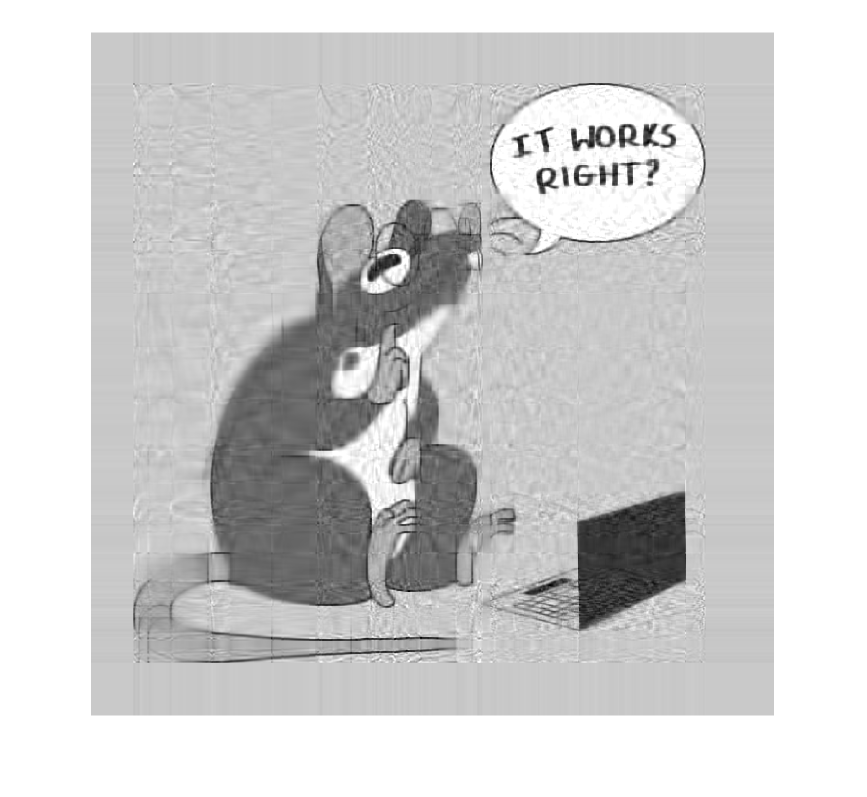
\includegraphics[width=0.5\linewidth]{figs/40_s_v.png}
    \caption{Image output using 40 singular values}
    \label{fig:40_s}
\end{figure}
\begin{figure}[h]
    \centering
    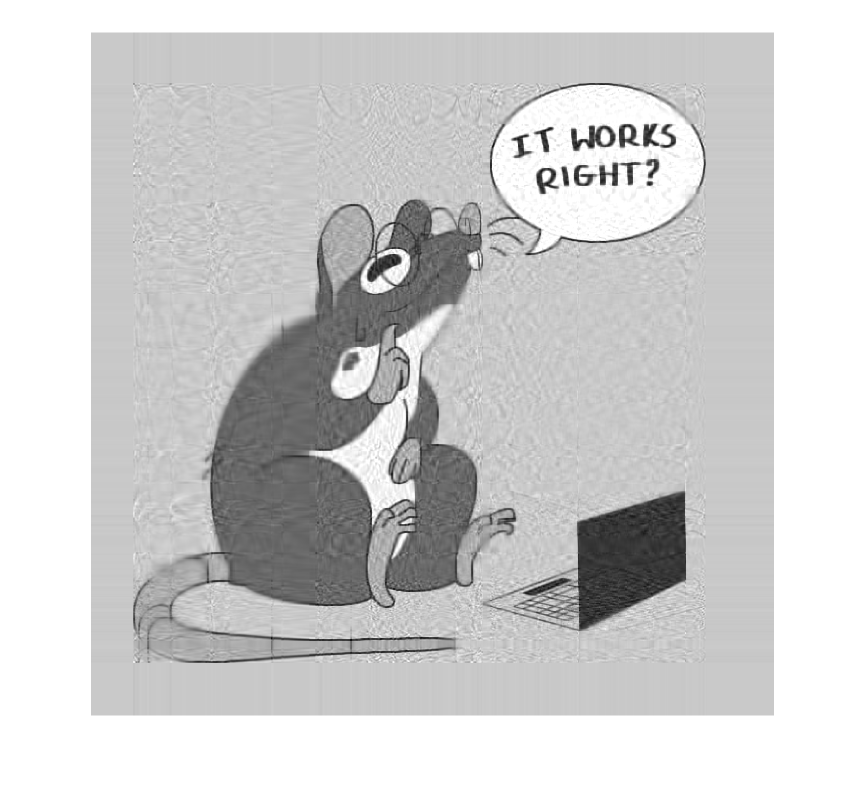
\includegraphics[width=0.5\linewidth]{figs/60_s_v.png}
    \caption{Image output using 60 singular values}
    \label{fig:60_s}
\end{figure}
\begin{figure}[h]
    \centering
    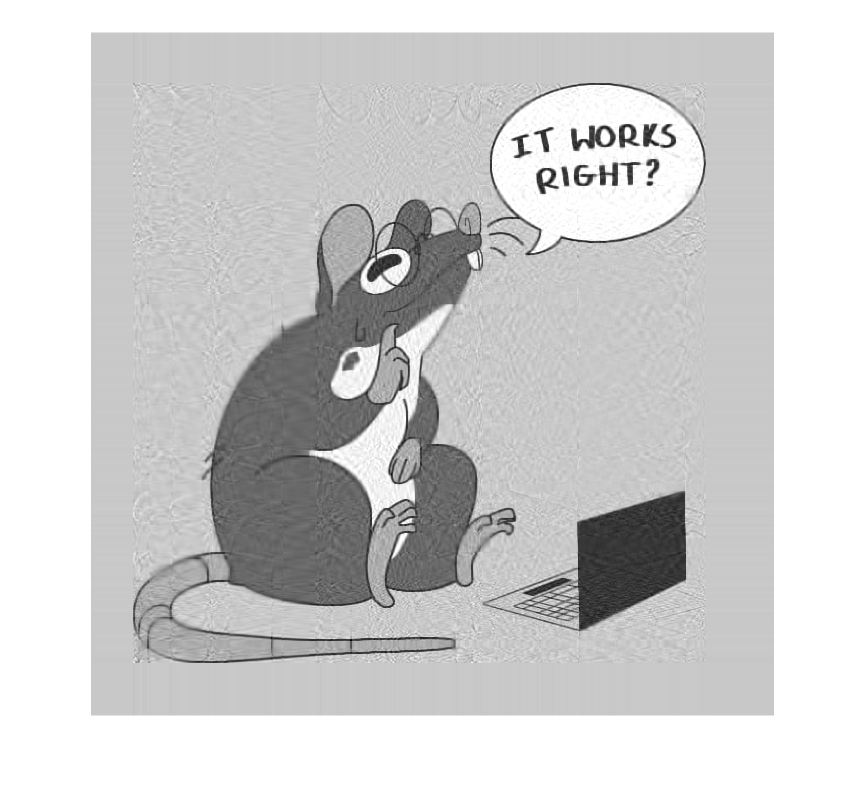
\includegraphics[width=0.5\linewidth]{figs/80_s_v.png}
    \caption{Image output using 80 singular values}
    \label{fig:80_s}
\end{figure}

As it was observed, 80 seems to be a minimum number of singular values needed
to obtain satisfying results. The image is clear and relatively similar to the original
one:
\begin{figure}
    \centering
    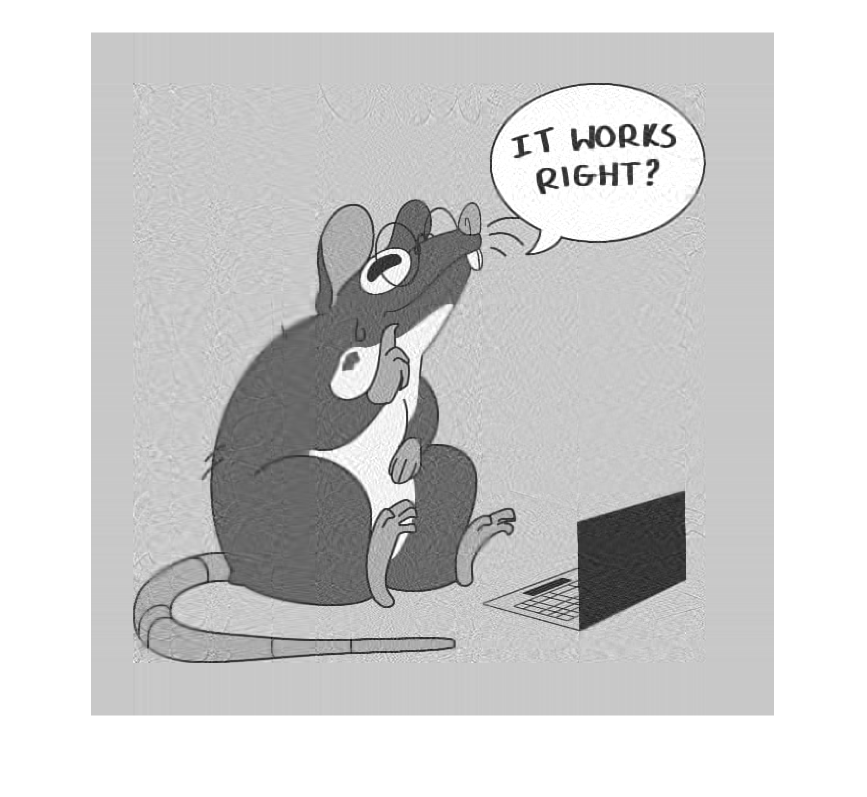
\includegraphics[width=0.5\linewidth]{figs/100_s_v.png}
    \caption{Image output using 100 singular values}
    \label{fig:100_s}
\end{figure}
